
\section*{Two-point distribution}

Consider $P_{ij}$ to follow the discrete \underline{two-point distribution}, where
\begin{align}
  \Prob(P_{ij}=x)=p \quad \mathrm{and} \quad \Prob(P_{ij}=y)=1-p.
\end{align}

We derive an expression the relative occurrence of reciprocal pairs $\varrho$ as
\begin{align}
\varrho = \frac{x+y}{\mu} - \frac{xy}{\mu^2}.
\end{align}

\begin{center}\vspace{1cm}
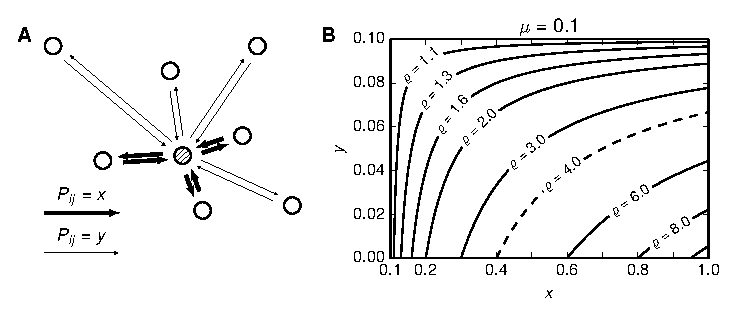
\includegraphics[width=0.9\linewidth]{two_point_full_figure.pdf}
\captionof{figure}{\textbf{A} Sketch of an network with connection probabilities $x$ and $y$ \textbf{B} For $\mu=0.1$ fixed, different pairings of $x$ and $y$ can induce high values of the relative occurrence of bidirectionally connected pairs $\varrho$. Dashed line marks an overrepresentation of $\varrho=4$ as observed for layer 5 pyramidal neurons in the rat visual cortex \cite{Song2005}.}
\end{center}\vspace{1cm}



